% implementation.tex

In this chapter we will cover our implementation process. It is structured in 4 parts. Part 1 consists of integrating ZooKeeper support and mechanisms into the Voldemort project, making Voldemort read from and store configurations in ZooKeeper. Part 2 contains our work towards rebalancing by the help of ZooKeeper. In part 3 we create the service Headmaster, which is a management service to run along side of the Voldemort. Headmaster keeps track of active nodes in the cluster and generates configuration for new nodes that are added at runtime. It also includes them in the current cluster and executes rebalances transfer resposibility to the new nodes. We have also created SigarAgent and StatusAnalyzer to allow for Headmaster to make management decisions based on recent node activity.

Lastly we have included a part 4 on how we wrote tests to validate our implementation during development.

\section{Part 1}
Integrating ZooKeeper into Voldemort and taking advantage of the coordination services ZooKeeper provides, proved rather difficult.
We chose to override and rewrite much of the current MetadataStore implementation to one that uses ZooKeeper as the backend storage engine instead of local files. 
Actual data is still of course stored locally, but configuration (metadata) now resides in the ZooKeeper cluster.
This abstraction works rather well for shared data files, but causes some issues with information that is stored for individual nodes. 
As such, we landed on a fixed path scheme, where certain configuration files are expected to reside on known locations, and will be presented later.

Using ZooKeeper as storage backend introduces a dependency of a running ZooKeeper cluster for normal operation of any node. While this is a liability and potential source for downtime in a highly available service, ZooKeeper is itself a highly available system and the 5 node setup is regarded as very stable and in heavy use at Yahoo\cite{zookeeperpaper}.In any case, the system will in general be able to operate through short ZooKeeper outages, as all meta and config data is cached locally, and will not affect operation. 

\subsection{Configuration}
Configuration is stored in a VoldemortConfig object. Normally this is created from settings stored in local files per node. At startup, the server looks for a properties file in a directory given by environment variable \texttt{VOLDEMORT\_HOME}. 

Now, if you specify a ZooKeeper connection URL as a command line parameter, the program looks for configuration in ZooKeeper.
We have given an example outline of the expected directory structure in Figure \ref{fig:configdirs}. This is for the three nodes \texttt{vold0.idi.ntnu.no}, \texttt{vold1.idi.ntnu.no} and \texttt{vold2.idi.ntnu.no}. You can see the expected path follows the pattern \texttt{/config/nodes/HOSTNAME/server.properties}. 

The startup code then reads and tries to parse the config file. If parsing fails, the server will fail to clearly signal something is wrong during startup, and needs immediate fixing. If the file is not found, the server registers a watch on the path in ZooKeeper. If there is a write to this file, ZooKeeper will let the server know and the config file can be re-read. 

One can argue whether to fail or listen when a config is not found, but we decided for the latter, to listen for changes, after implementing the management service. As we later will see, listening allows us to push new config files to a node by the help of our management daemon Headmaster. 

\begin{figure}[h]
\dirtree{%
.1 / \ldots{} \begin{minipage}[t]{8cm}(root directory)
			  \end{minipage}.
.2 config.
.3 nodes \ldots{} (individual node configs).
.4 vold0.idi.ntnu.no \ldots{} (hostname).
.5 server.properties.
.5 server.state.
.5 node.id.
.4 vold1.idi.ntnu.no.
.5 server.properties.
.5 server.state.
.5 node.id.
}
\caption{Individual node configs in the shared space.}
\label{fig:configdirs}
\end{figure}

Our modification inherits from the original VoldemortConfig object, so that the ZooKeeper capable version can be used in the same code, in the same manner. The modified code reads data from a fixed location in ZooKeeper, and sets the necessary settings and properties for the server to boot and join the cluster. The ZooKeeper connection URL is passed as a command line parameter.

The directory structure for the whole program can be viewed in its entirety in Figure \ref{fig:dirstruct}, and has been included for completeness.

\begin{figure}[h]
\dirtree{%
.1 / \ldots{} \begin{minipage}[t]{8cm}(The root can also be a chroot{.})
			  \end{minipage}.
.2 active .
.3 vold0.idi.ntnu.no \ldots{} (ephemeral).
.3 vold2.idi.ntnu.no \ldots{} (ephemeral).
.2 config \ldots{} (persistent) . 
.3 nodes (individual node configs).
.4 vold0.idi.ntnu.no.
.5 server.properties.
.5 server.state.
.5 node.id.
.4 vold1.idi.ntnu.no.
.5 server.properties.
.5 server.state.
.5 node.id.
.4 vold2.idi.ntnu.no.
.5 server.properties.
.5 server.state.
.5 node.id.
.3 cluster.xml.
.3 stores.xml.
.2 headmaster.
.3 headmaster\_0009 \ldots{} (ephemeral \& sequential).
.3 headmaster\_0011 \ldots{} (ephemeral \& sequential).
.3 headmaster\_0012 \ldots{} (ephemeral \& sequential) .
}
\caption{Directory structure in ZooKeeper. The nodes or directories are actually znodes and can hold data.}
\label{fig:dirstruct}
\end{figure}

\subsection{MetadataStore}
The internal state for a node is written to a \texttt{Store} called \texttt{MetadataStore}. It consists of an in memory cache store, and a persistent one on disk. The different stores are implementations of an abstract data \texttt{Store}. As such, we wrote a \texttt{Store} using ZooKeeper as the backend, and used this for persistent storage.

At startup we read the global configuration, the cluster and stores settings, from the Store. The Store fetches the requested files from ZooKeeper, and leaves a watch on the nodes. Because a store \emph{only} \emph{stores} data, the Store itself can not take advantage of the event deliveries from ZooKeeper: The Store keeps no application logic, and can be thought of as a hash map.

To notify and update the internal state of the node on events, we found it necessary to receive events in the configuration management logic, written in the \texttt{MetadataStore}.

When an event from the ZooKeeper client is delivered to the \texttt{MetadataStore}, we first sort it by type.
If it is a management event, like a disconnect event, we temporarily disable the ZooKeeper backend and serve data from the cache until it is reconnected. In our testing, such disconnects (session expiry) happened about once every hour, but the reconnect was usually done in less than two seconds. This instability may be due to our ZooKeeper cluster consisting of a single node and being on a different network.

After a session expiry, we receive a reconnected event when the ZooKeeper client reestablishes a connection. At this point, all set watches are lost, and all events during the connection loss will have been lost. We must therefore reset all watches and check the global configuration data on reconnect. 

\subsection{Handling the ZooKeeper connection}
Our way of handling of the ZooKeeper client and connection went through many stages and changes as we got a better understanding of its features.

Our currently preferred design can be viewed in \texttt{ActiveNodeZKListener}.
The ActiveNodeZKListener class wraps a ZooKeeper client connection, providing event delivery to the interface \texttt{ZKDataListener}. 
This approach removes a lot of the noise generated by the client, and delivers clear events that are simpler and clearer to handle and reason with when coding application logic.

We provide the following listener events:
\begin{description}

	\item[dataChanged(path):] 
		This method is called when data has been written to the watched znode on \texttt{path}.
	\item[nodeDeleted(path):] 
		A call to the listener to let it know the znode on \texttt{path} has been deleted.
	\item[reconnected():] 
		The connection handler provides a simple call \texttt{reconnected()} when a connection is reestablished after session expiry. When this call happens, we know it is safe to do sanity checking of our state and register watches again.
	\item[childrenList(path):]
		This one is a little bit special. This method is called whenever a znodes childrenList is changed. Recall that znodes are like nodes in a tree, and can have many children. This method call indicates new or removed children for the node on \texttt{path}.

\end{description}

We also include the possibility for receiving the raw events from the ZooKeeper client in the interface:

\begin{description}
	\item[process(event):]
		\texttt{Event} is the raw WatchedEvent from the ZooKeeper client. Registering as a \texttt{Watcher} will forward every internal ZooKeeper event to the listener.

\end{description}


\section{Part 2}

\subsection{Including rebalance functionality in Headmaster}
Voldemort uses external scripts for triggering rebalancing and repartitioning. This made incorporating this functionality into Headmaster very cumbersome. To get around this we created added the functionality of these scripts to Voldemort. We included two classes into the project: \texttt{RebalancePlannerZK} and \texttt{RebalancerZK}. These expose the methods: \texttt{createRebalacePlan()} and \texttt{rebalance(RebalancePlan plan)} used to trigger these events. Both classes utilize \texttt{ActiveZooKeeperListener} to fetch required configuration data from ZooKeeper. Headmaster now have access to these methods and can trigger them if deemed necessary. 

\subsection{Recursive triggered writes of meta data}
While adding the rebalance features, we bumped into an issue related to the architecture of Voldemort.
In a rebalance, the new config files are pushed (written) to each node separately using Voldemort admin data requests. This causes every node to execute a PUT of the new data on the MetadataStore.

As explained above, we use ZooKeeper for (persistently) sharing the global configuration files.
Also, we would like to be notified about changes to the config files using watches. So first you have N nodes in the cluster, executing N writes to the same file. Each file write potentially triggers N watches, causing a read and watch reset. Worst case we will end up with N writes and N*N watch triggers and reads, all in quick succession (less than a second).
We therefore decided to ignore such put requests in the ZooKeeper driven persistent Store, and only put the new data in the Metadata cache store, deferring the admin to use a ZooKeeper write operation to put the new config out, making the nodes do a re-read.


\begin{figure}[h]
    \centering
    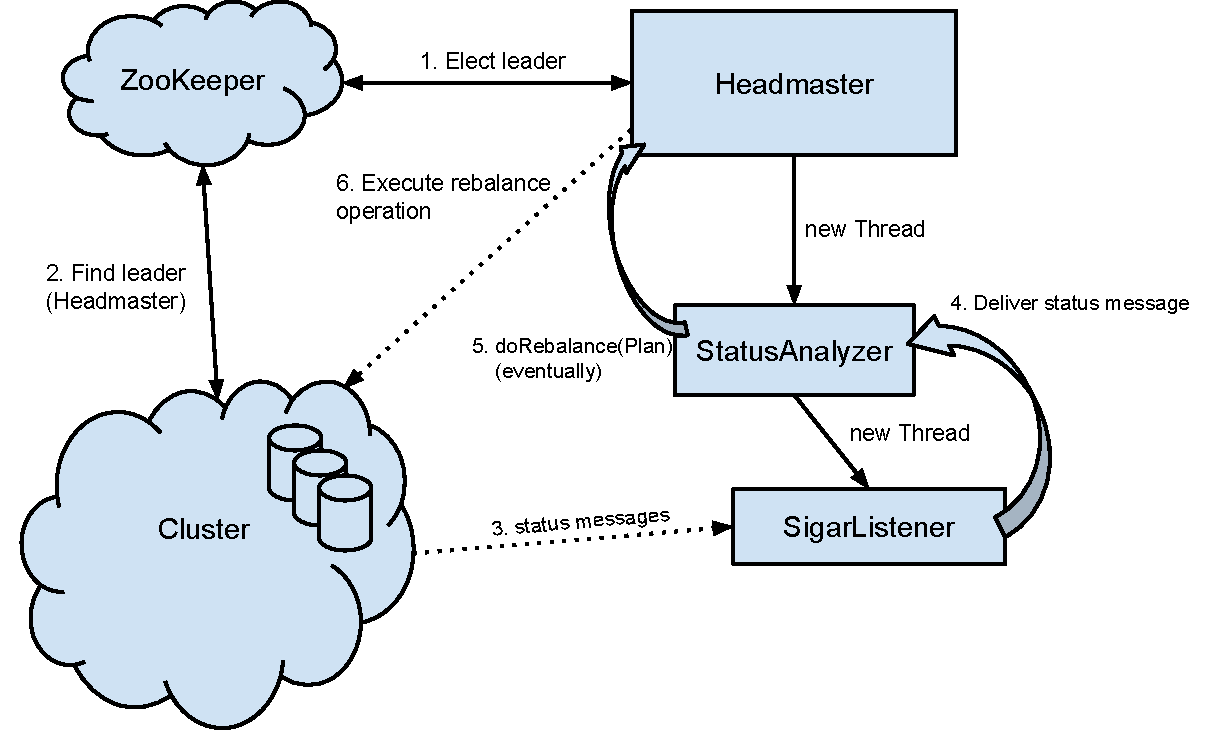
\includegraphics[width=1.0\textwidth]{implementation/Headmaster}
    \caption{System drawing of the management service Headmaster.}
    \label{fig:headmaster}
\end{figure}

\section{Part 3}
\subsection{Headmaster}
% We ran into some issues while writing these features. Originally the rebalance process sends the newly created \texttt{final\_cluster.xml} to all nodes. 

Headmaster is our clusters management service. It can be started on any node as long as ZooKeeper is reachable. When an instance of Headmaster is started an \emph{ephemeral} and \emph{sequential} znode is created on the path /headmaster in ZooKeeper. This means that each instance will automatically have its own sequence number appended to its name. So at runtime with 3 nodes running Headmaster we typically have a structure like in Figure \ref{fig:dirstruct}

Headmaster can be running on multiple nodes concurrently, and a leader election protocol based on ZooKeeper is responsible for only having one active Headmaster at the time. If the current Headmaster becomes unavailable, one of the waiting Headmasters will take over and become active. 

Whenever a node is starting Voldemort, the node registers itself under a znode called \texttt{/active} in ZooKeeper. This is done with the \emph{ephemeral} flag set. When a node creates this znode it also put its node id as the value. If the node has not yet received an id, it sets the value to ``NEW''. 

Through ZooKeeper, Headmaster is informed of all changes on the \texttt{/active} path. So, whenever there is a node registering, Headmaster checks for the value ``NEW''. Headmaster then checks if the node has an entry in the current \texttt{cluster.xml}. If the node has an entry, Headmaster simply changes the value to the correct id. If there is no entry in \texttt{cluster.xml}, Headmaster assigns the node a unique id and creates a znode under \texttt{/config/nodes/} and uploads the corresponding \texttt{server.properties} file. Finally \texttt{cluster.xml} is updated with a new entry for the new node. This node will not have responsibility for any partitions yet. A rebalance to give the newcomer a part of the keyspace can be triggered manually or by StatusAnalyzer will be presented below.

\subsection{SigarAgent}
SigarAgent is our service for monitoring activity on nodes in the cluster. Our solution is heavily inspired by the work of Andreas Baakind\cite{baakind}. We utilize Hyperic's sigar API to gather system information on each individual node and send this to Headmaster. We continuously send status on current CPU usage, memory used and how much data the node has stored compared to a given maximum. In contrast to Baakind who only informed his scaling service if any value was above a set threshold, we send a status message every 5 seconds. To prevent these messages for taking up too much resources, we use UDP instead of TCP as we do not require all messages to arrive at Headmaster. During all our testing we had 0 lost packages.

SigarAgent utilizes ZooKeeper to keep track of who is current Headmaster, and will react if there is a change of leadership. If there is no Headmaster active, SigarAgent will sleep until it is notified of a new Headmaster. 

\subsection{StatusAnalyzer}
StatusAnalyzer is a decision system available to the current Headmaster. StatusAnalyser receives status messages from all nodes running SigarAgent and stores them in a \texttt{HashMap<String, LinkedList<StatusMessage>>}. We store the last 10 messages received from each node, corresponding to 10 intervals of data. This HashMap is used to analyze the cluster state and trigger rebalancing actions if deemed necessary.

StatusAnalyser has a few useful member functions:

\begin{lstlisting}[style=customjava,label=lst:test,caption={Helper functions in StatusAnalyzer.}]

getAvgCPU(String hostname)
getCalmestNode()
analyzeCPU()
migratePartitions(List<String> strugglingNodes)

\end{lstlisting}

Every 30 seconds analyzeCPU is run to see if the average CPU-utilization of any node is over a threshold. We have defined a node running at over 84\% as a struggling node. If any nodes are above this threshold, getCalmestNode is run to see if there are any calm nodes . Any node with less than 70\% load is defined as a calm node. If any node is struggling and there is a calm node, migratePartitions is triggered. This will inform Headmaster that we need a rebalance action to stabilize the cluster. 

We have two strategies for moving partitions. If we have more than one struggling node we either pick a node at random and move one partition over to the calm node, or we move one partition from each struggling nodes over to the calm node. The former strategy will ensure a slow and steady transition while the latter could arrive at a stable state faster at the cost of performance during the more heavy rebalance. 

Figure \ref{fig:headmaster} gives an overview of the monitor/decision cycle and the typical ordering of events.

\section{Part 4}
\subsection{Testing}
When working on large projects, a lot of code lines are involved. To prevent breaking functionality underway, and to help verify correct (desired) behavior while working, we decided to write unit tests. 
Because of the complex series of events that need to happen while running the program to execute your desired code, it is much easier and more efficient to test and verify your code programmatically in a test environment. The design and verification of our Headmaster program greatly benefited from this approach. The event chain to test the code can be fairly complex, even though the application logic is fairly straight forward.

To create a test environment, we used JUnit and the Mockito project to mimic the behavior we need for validation.
Mockito is a testing framework for Java. It allows to create ``mock'' objects that can be used to trigger and verify program behavior in a predictable and controlled manner. The ``fake'', but controllable objects are very useful for eliminating outer dependencies, and instead having them behave in a completely predictable and controlled way.

Listing \ref{lst:mockito} shows a short example of how Mockito and JUnit is used to write short, simple yet powerful functional tests that verify behavior. It is also worth noting that the resulting test code is quite readable by a programmer.

\begin{lstlisting}[style=customjava,label=lst:mockito,caption={Test code utilizing Mockito. Think of the \texttt{@Mock} class as a subclass with all methods overrided \texttt{return null;}.}]
$$@Mock
ActiveNodeZKListener activeNodeZKListener;

Headmaster headmaster;

public void whenDataChangedTestIfWatchIsReset() {
    String path = "/config/cluster.xml";

    when(activeNodeZKListener.getStringFromZooKeeper(
    	path, true)).thenReturn(EXAMPLE_CLUSTER);

    headmaster.setZKListener(activeNodeZKListener);

    headmaster.dataChanged(path);

    /** 
     * verify method is called with params path, and watch flag set to true.
     */
    verify(activeNodeZKListener, times(1)).getStringFromZooKeeper(path, true);
}

\end{lstlisting}

Here we are verifying that upon receiving a notification that a znode has changed, the znode (path) is fetched with a new watch set.
All without actually providing a working third party object (ActiveNodeZKListener) to the test, the object is entirely faked with the static \texttt{when} and \texttt{thenReturn} methods. After setting the dependency class up with the desired behavior, it is injected into the class we are testing, then verify that the desired method is called once and only once (\texttt{times(1)}). Similarly it is easy to see how you can verify two calls (\texttt{times(2)}). For zero calls, it is recommended to use the more readable method \texttt{never}.
